\documentclass{beamer}

\usepackage[ngerman]{babel}
\usepackage[utf8x]{inputenc}
\usetheme{Dresden}
\useinnertheme{rounded}
\setbeamercovered{transparent}
\setbeamertemplate{footline}[frame number]
\beamertemplatenavigationsymbolsempty
%\usepackage{natbib}

\usecolortheme{seahorse}  % Sehr helles Blau
%\usecolortheme{dove}  % Glattes Weiß
%\usecolortheme{default}   


%%%%%%%%%%%%%%%%%%%%%%%%%%%%%%%%%%%%%%%%%%%%%%%%
\title[Projektseminar Robotik]{Projektseminar Robotik}
\subtitle[Hierarchische Karten]{Hierarchische Karten}
%\author[S. Wienert]{Stefan Wienert}
%%%%%%%%%%%%%%%%%%%%%%%%%%%%%%%%%%%%%%%%%%%%%%%%
\institute[Fak. Informatik -- HTW DD]{Fakultät Informatik\\ 
      Hochschule für Technik und Wirtschaft -- HTW Dresden}
\logo{\pgfimage[width=1cm]{material/htw.jpg}}

\titlegraphic{
\includegraphics[width=4cm]{material/stefanwienertlogo.png}}

\begin{document}

\frame{
    \titlepage
}
\frame{
    \frametitle{Inhaltsverzeichnis}
    \tableofcontents
}

\section{Zielstellung}
\begin{frame}{Zielstellung}

\begin{figure}[h]
 \centering
 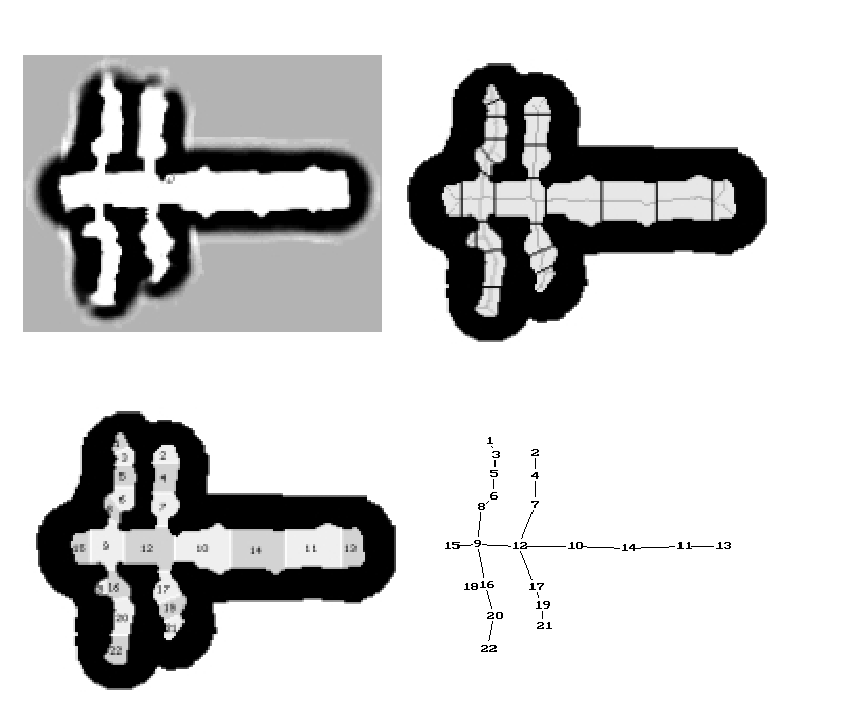
\includegraphics[width=0.6\textwidth]{./material/complete.png}
 % complete.png: 845x703 pixel, 72dpi, 29.81x24.80 cm, bb=0 0 845 703
 \caption{Übersicht \cite{Thrun1998}}
 \label{fig:gesamt}
\end{figure}


\end{frame}

\begin{frame}
 2 Möglichkeiten
 \begin{itemize}
  \item Verallgemeinertes Voronoi Diagramm \cite{Thrun1998}
  \item Thinning \cite{KoBangYun}, \cite{ZhangSuen}
 \end{itemize}

\end{frame}






\section{I. Voronoi-Diagramm}
\subsection{Grundlagen}
\begin{frame}{Voronoi-Diagramm}
 \begin{figure}[h]
 \centering
 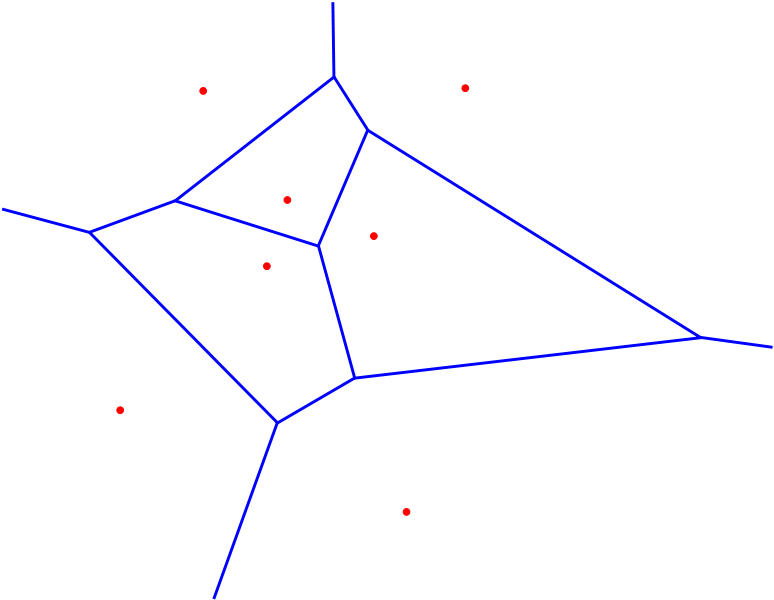
\includegraphics[width=0.4\textwidth]{./material/voronoi-step1-1.png}
 % complete.png: 845x703 pixel, 72dpi, 29.81x24.80 cm, bb=0 0 845 703
 \caption{Voronoi-Diagramm Wikipedia}
%  \label{fig:gesamt}
\end{figure}
\begin{description}
 \item[Voronoi-Diagramm] Linien in eine Punktwolke legen, so dass die Linien zu 2 Punkten immer denselben Abstand haben
 \item[Verallgemeinertes Voronoi-Diagramm] Statt der Punktwolke können auch Linien verwendet werden
\end{description}

\end{frame}

\subsection{Algorithmus}
\begin{frame}{Voronoi-Diagramm - 1. Berechnung des GVG}
  nach \cite{Thrun1998}

\begin{figure}[h]
 \centering
 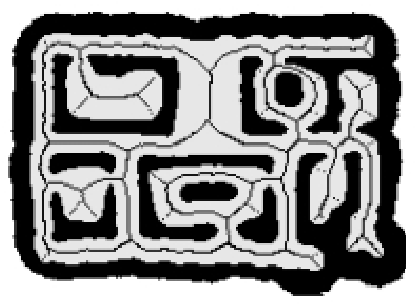
\includegraphics[width=0.6\textwidth]{./material/voronoi-step1.png}
 % complete.png: 845x703 pixel, 72dpi, 29.81x24.80 cm, bb=0 0 845 703
 \caption{Voronoi Schritt 1 \cite{Thrun1998}}
%  \label{fig:gesamt}
\end{figure}

% Voronoi Diagramm: 
% Verallgemeinertes Voronoi-Diagramm: Statt einfache Punkte können auch Linien verwendet werden
\end{frame}
\begin{frame}{Voronoi-Diagramm - 2. Kritische Linien}
\begin{figure}[h]
 \centering
 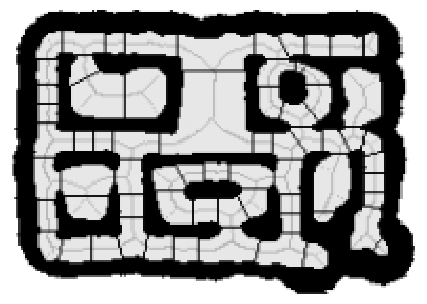
\includegraphics[width=0.6\textwidth]{./material/voronoi-step2.png}
 % complete.png: 845x703 pixel, 72dpi, 29.81x24.80 cm, bb=0 0 845 703
 \caption{Voronoi Schritt 2: Kritische Punkte/Linien \cite{Thrun1998}}
%  \label{fig:gesamt}
\end{figure}
Diejenigen Punkte auf dem Diagramm, die lokal einen geringen Abstand zur Wand besitzen
  
\end{frame}
\begin{frame}{Voronoi-Diagramm - Weitere Schritte}
 \begin{figure}[h]
 \centering
 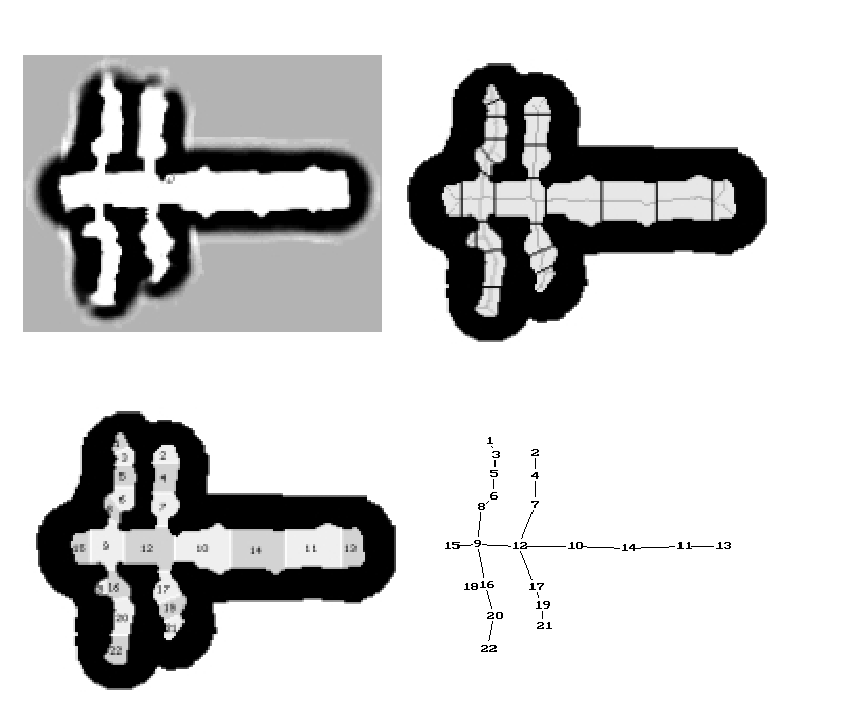
\includegraphics[width=0.65\textwidth]{./material/complete.png}
 % complete.png: 845x703 pixel, 72dpi, 29.81x24.80 cm, bb=0 0 845 703
 \caption{Übersicht \cite{Thrun1998}}
 \label{fig:gesamt}
\end{figure}
 
\end{frame}
\subsection{Probleme}
\begin{frame}{Probleme}
 \begin{itemize}
  \item Nachbarschaftssuche ist sehr aufwändig $\to$ sehr viele Papers mit Optimierungen
  \item Schwache Kreuzungen und Boundary Edges
 \end{itemize}
\begin{figure}[h]
 \centering
 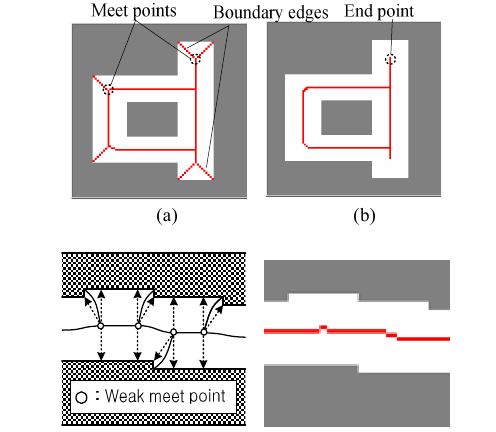
\includegraphics[width=0.5\textwidth]{./material/thinningvsvoronoi.png}
 % thinningvsvoronoi.png: 496x485 pixel, 72dpi, 17.50x17.11 cm, bb=0 0 496 485
 \caption{Voronoi vs. Thinning \cite{KoBangYun}}
 \label{fig:egal}
\end{figure}

 
\end{frame}

\section{II. Thinning/Skelettierung}
\begin{frame}{Thinning}
\begin{center}
 Idee: Man nehme den kompletten freien Raum (Flure, Räume), und wende darauf einen thinning-Algorithmus an.
 \bigbreak
 
 Dann bleibt ein Skelett, dem Voronoi sehr ähnlich, übrig.
 
 \end{center}
\end{frame}

\begin{frame}{Thinning}

\begin{figure}[h]
 \centering
 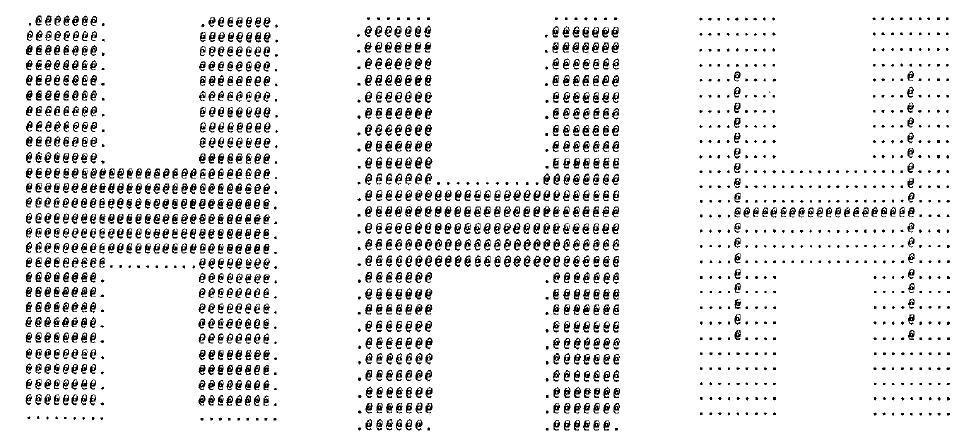
\includegraphics[width=0.65\textwidth]{./material/thinning1.png}
 % complete.png: 845x703 pixel, 72dpi, 29.81x24.80 cm, bb=0 0 845 703
 \caption{Thinning \cite{ZhangSuen}}
 \label{fig:gesamt}
\end{figure}
 
\end{frame}

\begin{frame}{Thinning-Bedingungen}

\begin{columns}\begin{column}[l]{0.4\textwidth}

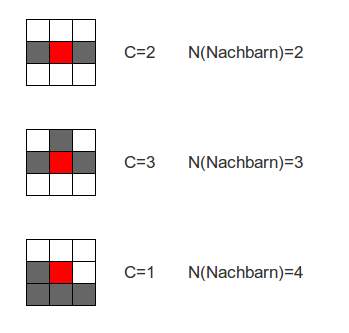
\includegraphics[width=1.0\textwidth]{./material/thinning2.png}

\end{column}\begin{column}[r]{0.6\textwidth}
 
 \begin{enumerate}
  \item Aktuelle Zelle ist belegt
  \item Connectivity $ = 1$
  \item $2 \leq $ Anzahl der Nachbarn $ \leq 6$
  \item Weitere Bedingungen nach Ausprägung des Algorithmus'
 \end{enumerate}
 
\end{column}\end{columns}
 
\end{frame}

\begin{frame}
 \centering
 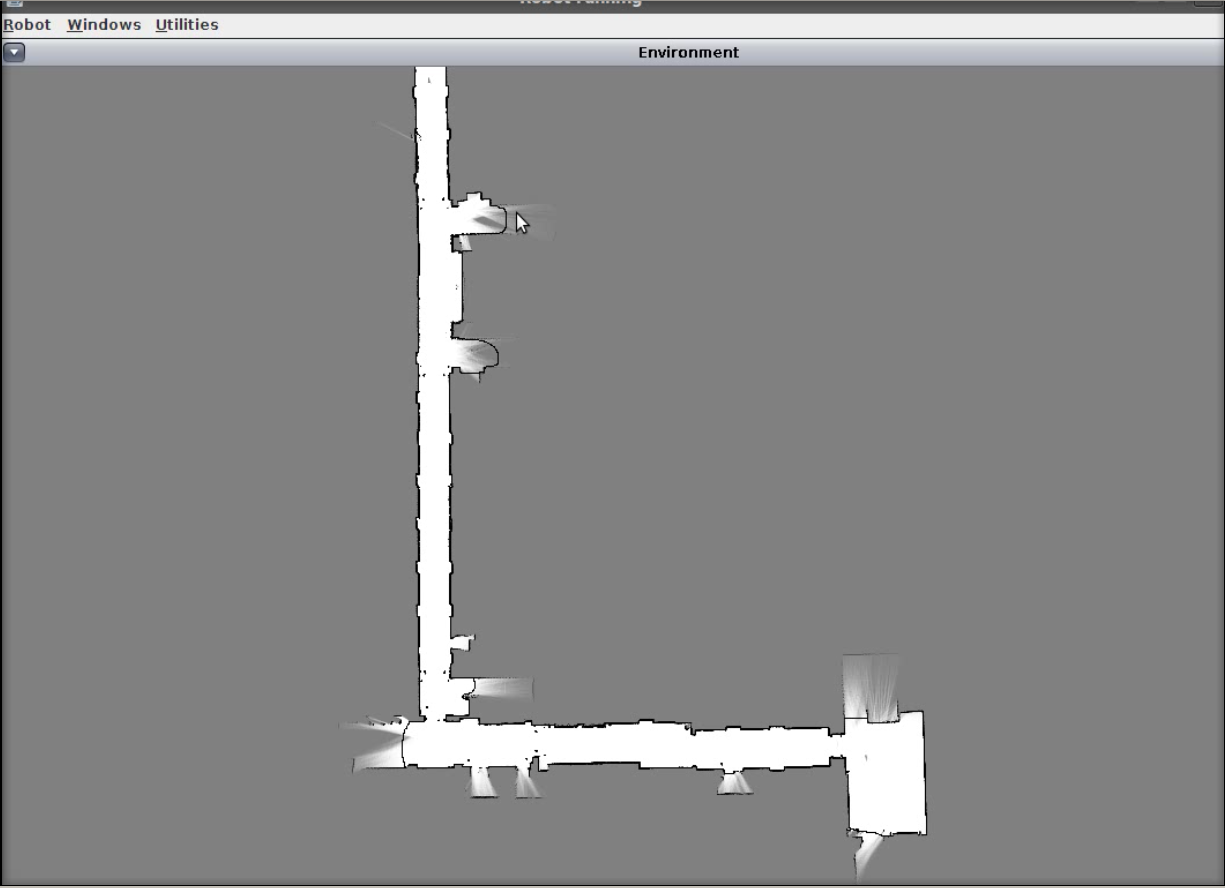
\includegraphics[width=0.85\textwidth]{./material/screencast.png}
\end{frame}


\section{Fazit/Offene Probleme}
\begin{frame}{Offene Probleme}
  \begin{itemize}
   \item Auffinden der kritischen Linien suboptimal
   \item Vorverarbeitung notwendig $\to$ stärkeres Smoothing, oder höherer Threshold
   \item Anpassung an Größe des Roboters entscheidend für Effektivität
   \item Tests mit weiteren Karten
  \end{itemize}
\end{frame}
\begin{frame}{Fazit zum Projektseminar}
  \begin{itemize}
   \item + Framework in Verbindung mit Java angenehm zu programmieren
   \item + interessante Aufgabe und viel Freiraum
   \item - Doku ist etwas verstreut im Wiki, teilweise mit Lücken
  \end{itemize}
\end{frame}



\frame{
  \frametitle{Literatur}
  \begin{thebibliography}{S. Thrun, 1998}

  \bibitem[S. Thrun, 1998]{Thrun1998}
    S. Thrun.	
    \newblock {\em Learning metric-topological maps for indoor mobile robot navigation}
    \newblock Artificial Intelligence 99/1, 1998.
  \bibitem[Zhang, Suen 1984]{ZhangSuen}
    Zhang, Suen
    \newblock {\em A Fast Parallel Algorithm for
Thinning Digital Patterns}
    \newblock Communications of the ACM, 03/1984 Vol.27 Nr. 3
    
  \bibitem[Ko, Song 2004]{KoBangYun}
    B-Y Ko, J-B Song
    \newblock {\em Real-time building of a thinning-based topological map with metric features}
    \newblock  Intelligent Robots and Systems, 2004. (IROS 2004) 2-2 okt. 2004   
  \end{thebibliography}

}

\end{document}
